% Drawing 148/01-16 -- folder 148, batch 01, archive page 18 (PDF page 19).
% Transcription: en bas à gauche, un tétraèdre vu par deux faces, dont la subdivision barycentrique est tracée en vert (les trois médianes de chaque face) ; un court chemin repassé en noir ; en pointillés rouges, avec des points rouges, une des cartes « carrés » associées.
% Kind: tetrahedron with barycentric subdivision of two faces, red dotted square map. Method 2 (schematic redraw from the facsimile). Status: partial.
% Notes: Colour render. Four vertices as dots; the outer edges thin, in brown; the edge common to the two visible faces heavy green. In heavy green, the three medians of each visible face, drawn through the computed centroid of the face and ending at the computed midpoints of the sides. A short heavy black stroke on the median of the right face above its centroid (the « chemin repassé en gras »). In red: a dotted line from the midpoint of the upper left edge across the left face to the midpoint of the common edge and on to the centroid of the right face and the midpoint of the right lower edge; a second dotted line across the lower part of the two faces; four red dots. Still differs: the red dotted lines and red dots are placed by eye and their path is partly a reading (they are faint and broken); the medians are drawn as exact medians, the page is freehand. Redrawn 2026-11-12 (issue 128): to check again.
% Coordinates: 1 unit = 1 mm = 1/100 of the crop width, y downwards as on the crop (bbox in page fractions: [0.2, 0.415, 0.5, 0.59]).
% Redrawn by Claude (claude-fable-5-2), issue #128, 2026-11-12; not checked by a human; not compiled (no TeX in the session).
% Rights: reproduces part of the work -- behind RENDER_TRANSCRIPTS, never published by itself.
\documentclass[tikz,border=3pt]{standalone}
\usepackage{amsmath,amssymb}
\usetikzlibrary{patterns,arrows.meta}
\tikzset{pencil/.style={black!45}, struck/.style={black!35}, mpt/.style={circle,draw,inner sep=1.3pt}, pt/.style={circle,fill,inner sep=0.9pt}, opt/.style={circle,draw,fill=white,inner sep=1.1pt}, Rd/.style={red!75!black}, Gn/.style={green!45!black}, Br/.style={brown!70!black}}
\begin{document}
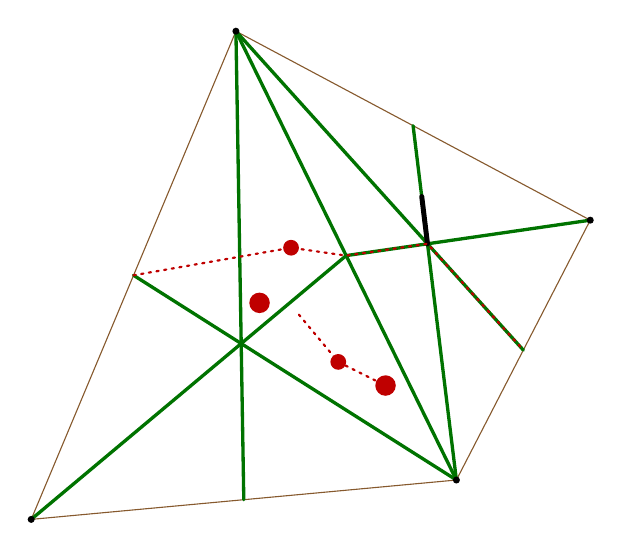
\begin{tikzpicture}[x=1mm,y=-1mm,line cap=round,line join=round,font=\small]
\coordinate (T) at (38,11);
\coordinate (R) at (83,35);
\coordinate (L) at (12,73);
\coordinate (B) at (66,68);
\coordinate (C) at (38.67,50.67);
\coordinate (D) at (62.33,38);
\coordinate (mLB) at (39,70.5);
\coordinate (mTL) at (25,42);
\coordinate (mTB) at (52,39.5);
\coordinate (mTR) at (60.5,23);
\coordinate (mBR) at (74.5,51.5);
\draw[Br] (T) -- (L) -- (B) -- (R) -- cycle;
\draw[Gn,very thick] (T) -- (B);
\draw[Gn,very thick] (T) -- (C) -- (mLB);
\draw[Gn,very thick] (L) -- (C) -- (mTB);
\draw[Gn,very thick] (B) -- (C) -- (mTL);
\draw[Gn,very thick] (T) -- (D) -- (mBR);
\draw[Gn,very thick] (R) -- (D) -- (mTB);
\draw[Gn,very thick] (B) -- (D) -- (mTR);
\draw[line width=1.8pt] (D) -- (61.6,32);
\draw[Rd,dotted,thick] (mTL) -- (45,38.5) -- (mTB) -- (D) -- (mBR);
\draw[Rd,dotted,thick] (46,47) -- (51,53) -- (57,56);
\fill[Rd] (41,45.5) circle [radius=1.3];
\fill[Rd] (45,38.5) circle [radius=1];
\fill[Rd] (51,53) circle [radius=1];
\fill[Rd] (57,56) circle [radius=1.3];
\node[pt] at (T) {};
\node[pt] at (R) {};
\node[pt] at (L) {};
\node[pt] at (B) {};
\end{tikzpicture}
\end{document}
